\chapter{周期势与计算方法}
能带理论是凝聚态物理中最重要的理论之一,它是量子力学确立后,在研究金属电导理论过程中发展起来的,已经成为固体电子理论的支柱。理想晶体的原子有序排列成晶格,具有平移周期性,势能$V(\vec r)$满足:
\begin{equation}\label{eq:solid-2}
	V(\vec r)=V(\vec r+\vec R_n)\quad\mbox{($\vec R_n$为任意格矢)}
\end{equation}
\textrm{Bl\"och}定理指出:
{\it 对于具有周期性的势场,单电子的Schr\"odinger方程}
\begin{equation}\label{eq:solid-1}
  \biggl[-\dfrac{\hbar^2}{2m}\nabla^2+V(\vec r)\biggr]\psi=E\psi
\end{equation}
{\it 的解满足}
\begin{equation}
  \psi(\vec r+\vec R_n)=e^{i\vec k\cdot\vec R_n}\psi(\vec r)
  \label{eq:bloch}
\end{equation}
$k$是与平移对称性相应的量子数,因此理想晶体的电子波函数除了与势函数具有相同的平移周期性,还受到平面波的相位控制。密度泛函理论发展起来之后,为包括能带计算在内的电子结构模拟提供了坚实的基础,可以通过选定交换-相关泛函(主要是LDA或GGA),自洽迭代求解Kohn-Sham方程直接得到电子能带。在具体应用DFT求解能带时,除了泛函的选择,还需要考虑各种近似,不同近似方法的差别在于单电子有效势和波函数形式的选取两方面。

\section{Muffin-Tin近似与非Muffin-tin校正}
周期体系的势函数与一般原子、分子不同,集中在原子间区域,波函数较为平缓,并且有周期特征,如图\ref{Potential-Wave}所示:
\begin{figure}[h!]
\centering
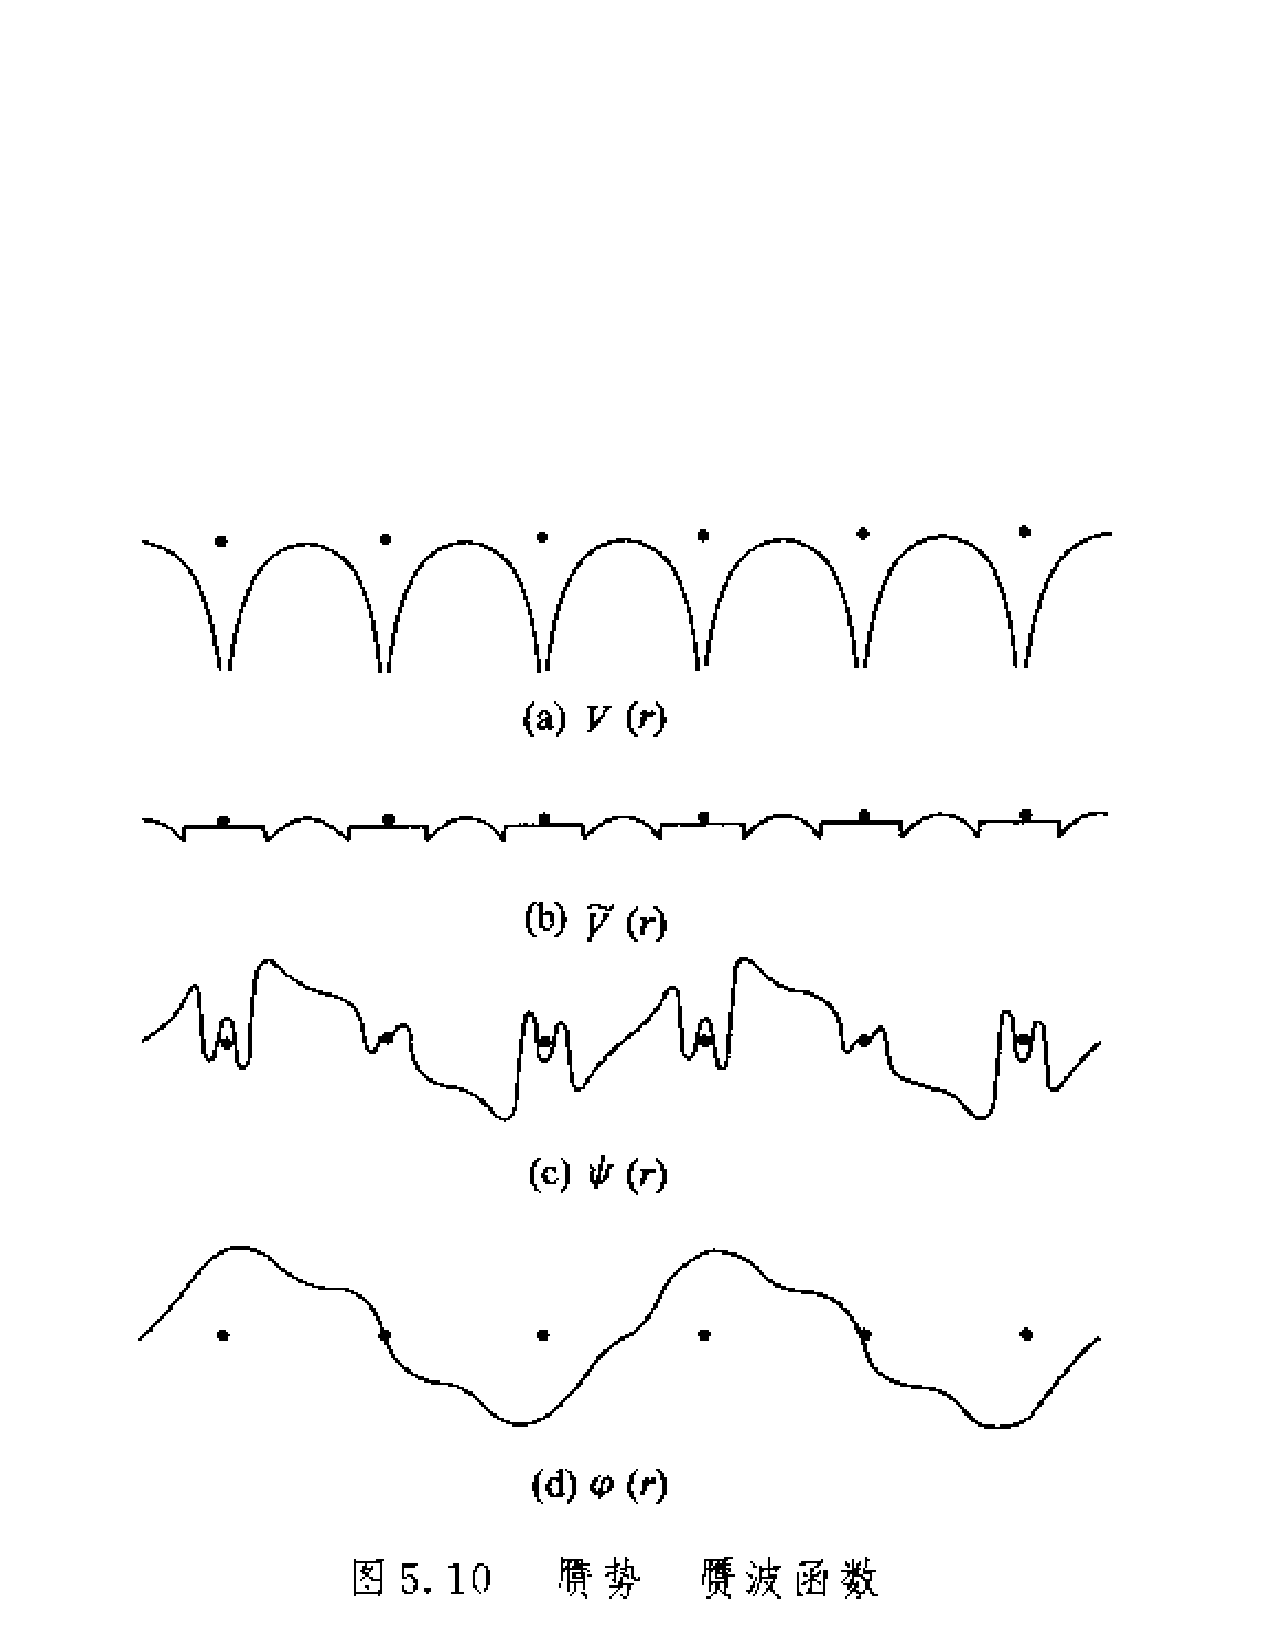
\includegraphics[height=0.8in,width=4.in,viewport=41 458 539 546,clip]{Pseudo_wave.pdf}\\
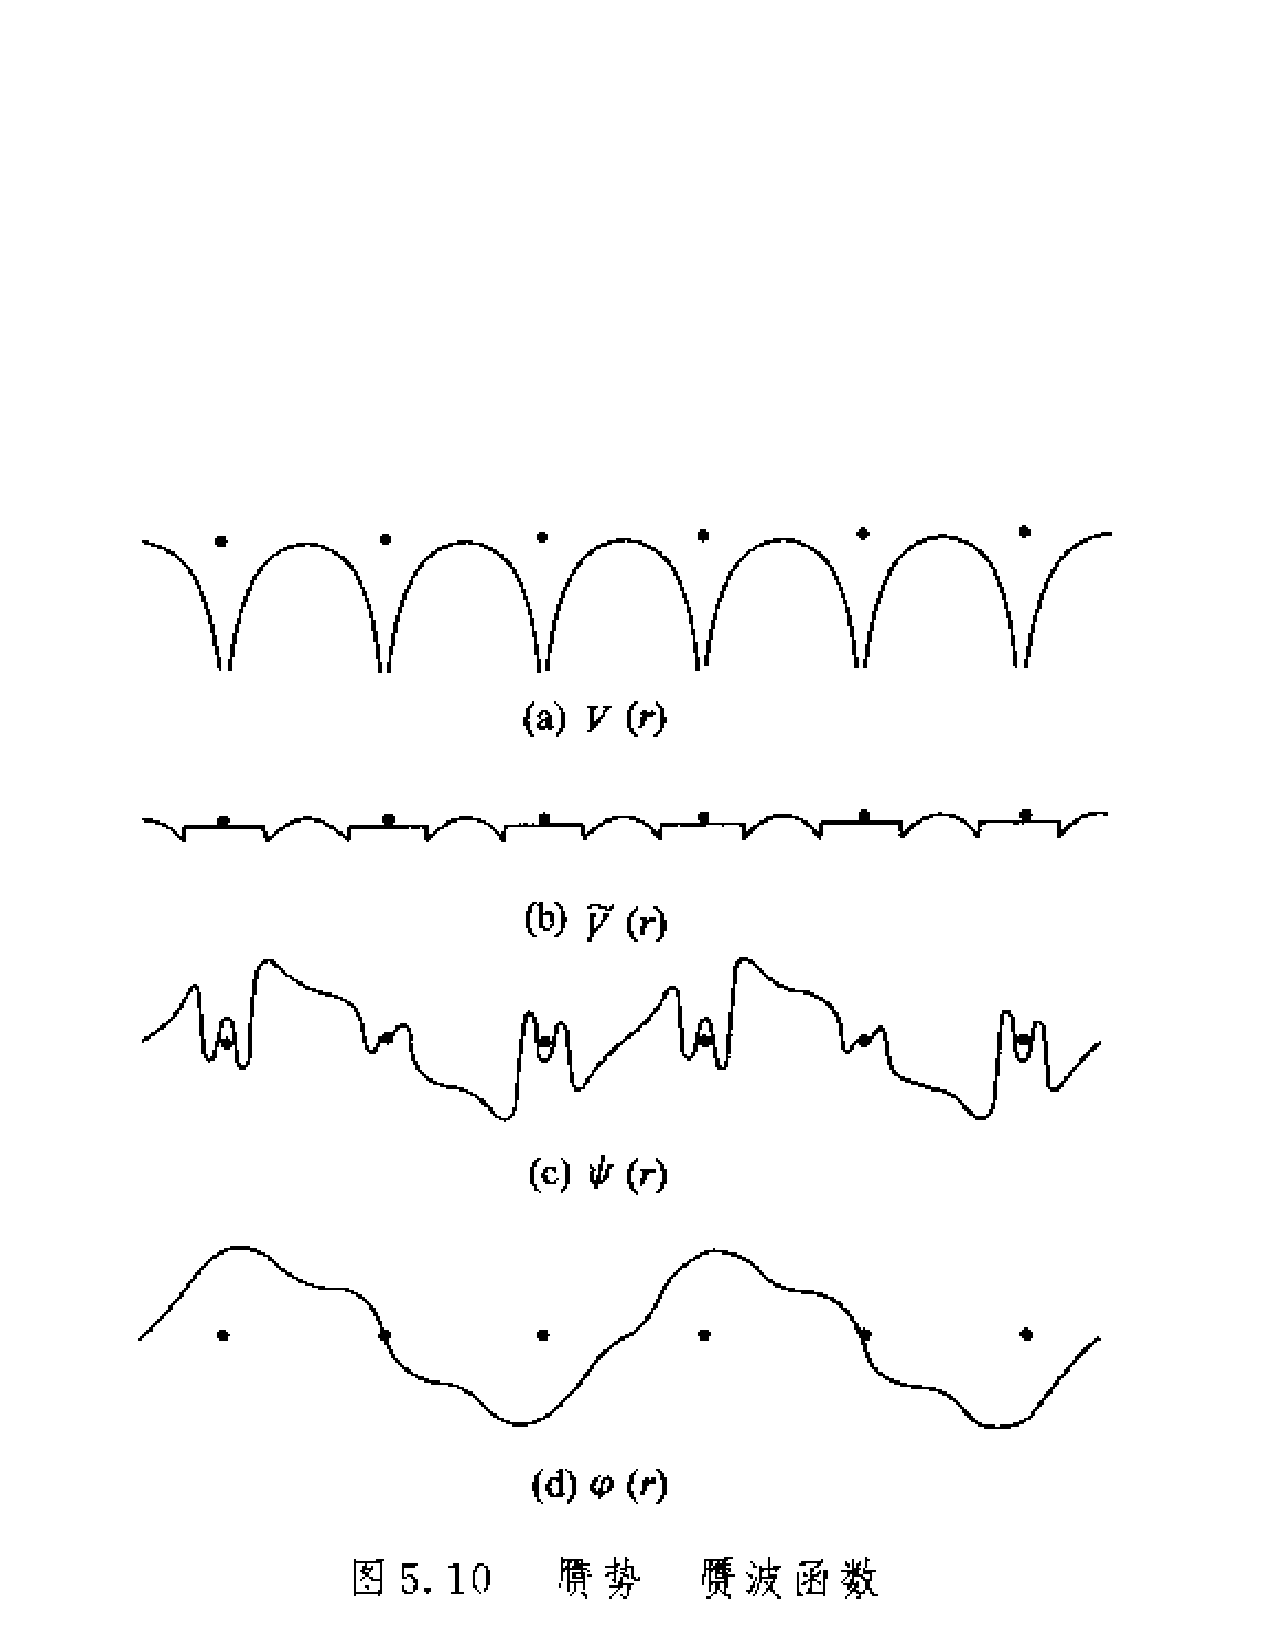
\includegraphics[height=0.8in,width=4.in,viewport=41 238 539 339,clip]{Pseudo_wave.pdf}
\caption{\small \textrm{The periodic Potential (up) and the wave functions (down) in crystal.}}%(与文献\cite{EPJB33-47_2003}图1对比)
\label{Potential-Wave}
\end{figure}
最早的能带计算方法是Wigner-Seitz(WS)原胞方法\cite{PR43-804_1933},没有特别考虑周期特征。该方法假定晶体势场有球对称性,即$V(\vec r)=V(r)$,波函数为中心力场Schr\"odinger方程标准的线性组合,边条件为$\left(\dfrac{\partial\psi_{\vec k}(r)}{\partial r}\right)_{r_0}$,$r_0$为球半径。该方法在碱金属能带计算取得了很大的成功。将原胞简化为球,结果仅依赖于每个原子平均占据的体积,忽略实际晶体结构的影响。如果采用真实的多面体WS原胞,为了满足表面边边界条件,计算将变得十分复杂,同时也会导致中心力场在原胞边界上导数的不连续。为了克服WS原胞方法的缺陷,1937年,Slater提出Muffin-Tin(MT)近似\cite{PR51-846_1937}。MT近似的主要思想是将WS原胞分为两个区域,一个是以原胞中的每个原子{\it i}\,为中心,半径为$r_i$的彼此不相交叠的球形区,此区域内具有球对称性势$V(r_i)$,在接近原子核区域,势能变化非常较大;球形区以外为第二部分(间隙区),此处势能近似为一常数,如图\ref{Muffin_tin-1}所示:
\begin{figure}[h!]
\centering
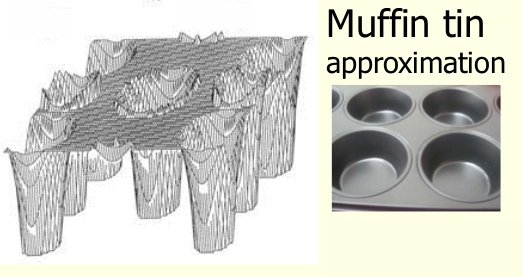
\includegraphics[height=1.45in,width=1.92in,viewport=1 22 317 295,clip]{Muffin-tin.png}
\includegraphics[height=1.45in,width=1.92in,viewport=1 20 515 435,clip]{Muffin-Tin.png}
\caption{\small \textrm{Division of the unit cell into spheres(I) and into interstitial region(II)}}%(与文献\cite{EPJB33-47_2003}图1对比)
\label{Muffin_tin-1}
\end{figure}

\begin{equation}
  V(\vec r)=\left\{
  \begin{aligned}
    &V(r),\quad&r\leqslant R_{MT} \\
    &V_c.&r>R_{MT}
  \end{aligned}\right.
  \label{eq:Muffin-Tin}
\end{equation}
为简化计算,通常取$V_c$=0,这等价于将晶体的势能零点移动到$V_c$位置上。MT势比原胞法相更接近实际情况,适用性更强,即使对于晶体势场不能完全用MT势描述的情况,如球内的非球形对称部分不能完全忽略的情况,也可以通过适当的方法修正。

为了计算周期性晶体势场,Mattheiss提出了一个构造MT势的方法,在中心原子的势场上叠加上周围原子势场以中心为原点的球谐函数展开的球对称部分\cite{PRA133-1399_1964}。将Coulomb势和交换项分开处理。Coulomb势用晶体中原子势的静电排斥叠加表示,临近原子的Coulomb势叠加用L\"owdin发展的$\alpha$展开方法计算:
\begin{equation}
  V_C(r)=\sum_i\dfrac{N_i}{2a_ir}\int_{|a_i-r|}^{|a_i+r|}r'V_C^{at}(r')dr'
  \label{eq:lodin-alpha}
\end{equation}
其中$a_i$是第$i$个等同原子球的半径;$N_i$是第$i$个原子的等同原子球数目;$V_C^{at}(r)$是原子的Coulomb势,可用下式%\eqref{eq:atomic-coulomb}
计算:
\begin{equation}
  V_C^{at}(r)=-\dfrac{2Z}r+\frac2r\int_0^r4\pi\rho^{at}(r')r'^2dr'+2\int_r^{\infty}4\pi r'\rho^{at}(r')dr'
  \label{eq:atomic-coulomb}
\end{equation}
其中$\rho^{at}(r)=\sum\limits_l n_lu_l^2$是自洽的原子电荷密度,$n_l$是占据电子数,$u_l$是自洽原子波函数\cite{Herman-Skillman}。对于含有重元素的体系,$u_l$的计算可参考文献\inlinecite{PR137-23_1965}。由此得到的MT势为
\begin{equation}
  V_{MT}(r)=V_C^{at}(r)+\sum_i\dfrac{N_i}{2a_ir}\int_{|a_i-r|}^{|a_i+r|}r'V_C^{at}(r')dr'+V_{xc}(r)-V_c
  \label{eq:potential-MT}
\end{equation}
最初的交换势$V_{xc}$贡献用Slater的$\chi_{\alpha}$方法计算\cite{PR81-385_1951},现在则根据选定的交换-相关泛函给出。计算时$\rho(r)$取晶体的空间电荷密度,初始值为中心原子的电子密度叠加相邻原子的电子密度。$V_c$是MT球间常数势。对单原子金属体系,WS原胞内的MT球间常数势为
\begin{equation}
  V_c=\dfrac3{R_{WS}^3-R_{MT}^3}\int_{R_{MT}}^{R_{WS}}V_{MT}(r)dr
  \label{eq:monoatomic-ini}
\end{equation}
这里$R_{WS}$由$(4/3)\pi R_{WS}^3=\Omega_0$计算得到,$\Omega_0$是原胞体积。

MT近似方法主要适用于具有密堆积的简单晶格的单原子(过渡)金属\cite{SSP26-104_1971},但对于非密堆积的金属化合物(如体心立方的CsCl结构)\cite{PRB13-5362_1976}的计算结果不理想,因为在化合物中原胞电中性条件无法保证。对于这类含有复式晶格的体系,必须采用另外的方法计算\cite{PSSB36-447_1969}。
%与简单晶格计算方法相比,复式晶格计算中叠加的是位于不同中心的电子密度而不再是原子势,并利用元胞的电中性假设,求出MT球间的常数电荷。确定电荷密度之后,利用Poisson方程求解MT球内势能和球间的常数势$V_c$。

%复式晶格的电子密度表示
%\begin{equation}
%  \rho_s(r)=\rho_s^{at}(r)+\sum_{mj}\dfrac{n_{mj}}{2a_{mj}r}\int_{|a_{mj}-r|}^{|a_{mj}+r|}\rho_m^{at}(r')r'dr'
%  \label{eq:equation-58}
%\end{equation}
%这里$\rho_s^{at}(r)$是$s$原子的电子密度;$r=|\vec r-\vec{\tau}_j|\leqslant R_{MT}^s$;$\vec{\tau}_j$是第$j$个等同原子球心位置;$n_{mj}$是中心在$\tau_j$矢径为$a_{mj}$的等同原子$m$的数目。WS原胞MT球外的常数电荷由复式原胞的电中性条件确定。
%\begin{equation}
%  \rho_c=\dfrac{\sum_i(Z_i-Q_i)}{\Omega_0-\sum_i\Omega_i}
%  \label{eq:solid-59}
%\end{equation}
%其中$Q_i=4\pi\int_0^{R_i}\rho_i(r)r^2dr$,$\Omega_i$是球心位于$\vec{\tau}_i$的球体积。在复式晶格内,根据周期性边界条件求解Poisson方程得到球对称晶体势,并对角度求和
%\begin{equation}
%  \begin{split}
%   V_s(r)=&-\frac{2Z_s}r+\frac{8\pi}r\int_0^r\rho_s(r')r'^2dr'+8\pi\int_r^{R_{MT}^s}\rho_s(r')r'dr' \\
%   &-2\sum_j(Z_j-Q_j+\rho_c\Omega_j)\varphi(\vec{\tau}_j-\vec{\tau}_s)-4\pi\rho_c(R_{MT}^s)^2 \\
%   &+\frac{(4\pi)^2}{3\Omega_0}\sum_j\int_0^{R_{MT}^s}[\rho_j(r')-\rho_c](r')^4dr'
%  \end{split}
%  \label{eq:solid-60}
%\end{equation}
%MT间的常数势根据式\eqref{eq:solid-61}确定:
%\begin{equation}
%  \begin{split}
%    V_c=&\frac2{\Omega_0-\sum_j\Omega_j}\left[\frac32\sum_j\frac{\Omega_j}{R_j}\left(Z_j-Q_j+\frac56\rho_c\Omega_j\right)\right.\\
%    &+\left.\sum_{ij}\Omega_j(Z_i-Q_i+\rho_c\Omega_i)\varphi(\vec{\tau}_i-\vec{\tau}_j)\right] \\
%    &+\frac{(4\pi)^2}{3\Omega_0}\sum_j\int_0^{R_{MT}^s}[\rho_j(r')-\rho_c](r')^4dr'
%  \end{split}
%  \label{eq:solid-61}
%\end{equation}
%这里$\varphi(\vec{\tau}_i-\vec{\tau}_j)$是位于$\vec{\tau}_j$的$j$离子静电势;$R_{MT}^s$是第$s$个MT球的半径。该球内的势能
%\begin{equation}
%  V_{MT}^s(r)=V_s(r)+V_{xc}(r)-V_c
%  \label{eq:solid-62}
%\end{equation}

%此外,晶体中离子(实)间的相互作用用Madelung势表示,对大多数晶体来说,晶体的Madelung势是已知的。需要指出的是,采用MT近似计算,正确选择MT球半径非常重要,因为球半径选择对于势能的Coulomb势和MT球内的电子电荷有重要影响。%对于WS原胞内含有两个原子的体系,MT球半径的选择使得两个MT球相切位置的MT势\eqref{eq:solid-62}相等。

使用MT近似方法,MT球外的势能是一常数,但实际上要求%如果MT球外有非零的电子密度,无法通过MT近似构造出与此电荷密度一致的势能。假设MT球外的电荷满足式\eqref{eq:solid-59},
求解Possion方程所得到的势能$V_c$并非是一常数,而与位置有关。所以应用MT近似,假设$V_c$为一常数,是MT近似误差的主要来源。

%\subsection{非MT校正}
关于MT近似的改进方法有许多\cite{RPP44-139_1981}。考虑对MT近似的修正,主要有两类方案。一种是在推导Hamiltonian的基函数时考虑非MT效应;另一种采用MT近似构造基函数,但对势能进行非MT修正。一般来说主要应用第二种方案,构造一般形式的势能。在MT近似下,WS原胞分为球形区(S)和间隙区(I)两部分。对这两部分区域,非MT校正分别采用了不同形式的校正形式。一般地,在MT球内,晶体势用球谐函数(或者是满足晶体对称性的球谐函数),MT球外的势能用Fourier级数展开\cite{PRB13-5362_1976}
\begin{equation}
  V(\vec r)=\left\{
  \begin{aligned}
    &\sum_LV_L(r)Y_L(\hat{\vec r}),\quad &r\leqslant R_{MT}\\
    &\sum_{\vec G_n}V_I(\vec G_n)e^{i\vec G_n\cdot\vec r},&r>R_{MT}
  \end{aligned}\right.
  \label{eq:solid-63}
\end{equation}
这里$L\hat=l,m$,$\vec G_n$为倒格矢,$Y_L(\vec r)$是球谐函数。%这是合理的修正,因为靠近原子核,势能具有原子型势能特征。在MT球外,要求满足Bloch函数边界条件特征。由于MT球内外的势能表象不同,因此要求势能在MT球表面连续。
为求解交换-相关势$V_{xc}$,将电荷密度也采用类似的形式展开。由此得到晶体势
\begin{equation}
  V(\vec r)=V_{MT}(\vec r)+V_{WMT}(\vec r)+V_{NS}(\vec r)
  \label{eq:solid-64}
\end{equation}
这里$V_{MT}(\vec r)$是简单的MT势;$V_{WMT}(\vec r)$表示MT球外势能Fourier展开对MT近似常数势的偏离;$V_{NS}(\vec r)$是式\eqref{eq:solid-63}第一个求和项中所有$\nu$$\neq$0之和。根据式\eqref{eq:solid-63},$V_{WMT}(\vec r)$仅在MT球外非零,球内为零;而$V_{NS}(\vec r)$只在MT球内有非零值。

研究表明,对于过渡金属和具有密堆积结构的过渡金属化合物,间隙区势能近似为常数,因此MT方法是很好的近似,计算结果只会有很小的误差\cite{PR153-931_1967,PRB1-1318_1970,PLA33-414_1970}。计算也表明,一般$V_{WMT}(\vec r)$比$V_{NS}(\vec r)$大得多。

%\section{能带计算方法}
晶体电子结构的计算可以分为两个部分:构造合理的具有平移周期性的晶体势场;在该势场下求解Schr\"odinger方程。不同的能带计算方法的主要区别在于:
\begin{itemize}
	\item 基函数的选取的不同
	\item 根据研究对象性质的不同对晶体的势能作合理的近似
\end{itemize}
不同的计算方法,主要通过基函数为特征命名。

\section{基态总能量表达式}
基态总能量表达式\footnote{这部分主要参阅文献\inlinecite{XIE-LU}}
在DFT框架内,周期体系的总能量$E_T$由晶格中的电子能量$E_{e-e}$与离子实排斥能$E_{N-N}$之和:
	\begin{equation}
		E_T=E_{e-e}+E_{N-N}=T[\rho]+E_{ext}+E_{\mathrm{Coul}}+E_{\mathrm{XC}}+E_{N-N}
	\end{equation}
根据\textrm{Kohn-Sham}方程,其中动能泛函用单电子能量表示为
\begin{equation}
	T[{\rho}]=\sum_in_i\langle\psi_i|\varepsilon_i-V_{\mathrm{KS}}|\psi_i\rangle
\end{equation}
$n_i$是$\psi_i$上的电子占据数,$\varepsilon_i$是其能量本征值,因此有
\begin{equation}
	E_T=\sum_in_i\varepsilon_i-\dfrac12\int\int\mathrm{d}\vec r\mathrm{d}\vec r\dfrac{\rho(\vec r)\rho(\vec r^{\prime})}{|\vec r-\vec r^{\prime}|}+\int\mathrm{d}\vec r\rho(\vec r)[\epsilon_{\mathrm{XC}}(\vec r)-V_{\mathrm{XC}}(\vec r)]+E_{N-N}
\end{equation}

周期体系的总能量表达式在动量空间($\vec K$空间)计算更方便
\begin{equation}
	E_T=\textcolor{red}{\sum_in_i\varepsilon_i}-\dfrac{\Omega}2\sum_{\textcolor{red}{\vec k\neq 0}}\rho^{\ast}(\vec k)V_{\mathrm{Coul}}(\vec k)+\Omega\sum_{\vec k}\rho^{\ast}(\vec k)[\epsilon_{\mathrm{XC}}(\vec k)-V_{\mathrm{XC}}(\vec k)]+E_{N-N}
\end{equation}
其中$V_{\mathrm{Coul}}(\vec k)$、$\epsilon_{\mathrm{XC}}(\vec k)$与$\rho^{\ast}(\vec k)$分别是\textrm{Coulomb}相互作用、单个电子的交换-相关能、交换-相关势和电子密度的\textrm{Fourier}分量。

电子间的\textrm{Coulomb}相互作用由\textrm{Poisson}方程计算
\begin{equation}
	\nabla^2V_{\mathrm{Coul}}(\vec r)=-4\pi\rho(\vec r)
\end{equation}
其\textrm{Fourier}展开为
\begin{equation}
	V_{\mathrm{Coul}}(\vec k)=\dfrac{4\pi\rho^{\ast}(\vec k)}{|\vec k|^2}
\end{equation}
交换-相关势和交换-相关能的计算一般先在实空间计算$\epsilon_{\mathrm{XC}}(\vec r)$和$V_{\mathrm{XC}}(\vec r)$后,再通过\textrm{Fourier}变换到动量空间,得到$\epsilon_{\mathrm{XC}}(\vec k)$和$V_{\mathrm{XC}}(\vec k)$

离子间\textrm{Coulomb}相互作用能之和
\begin{equation}
		E_{N-N}=\dfrac12\sum_{\vec R,s}\sideset{}{^{\prime}}\sum_{\vec R^{\prime},\vec s^{\prime}}\dfrac{Z_sZ_{s^{\prime}}}{|\vec R+\vec r_s-\vec R^{\prime}-\vec r_s^{\prime}|}
\end{equation}
这里$Z_s$是离子实的电荷数,$\vec R$表示晶格点的位矢,$\vec r_s$代表元胞内原子的相对位矢。

\textcolor{red}{\textbf{注意}}:~$E_{N-N}$求和包含无穷多项,是发散的;$V_{\mathrm{Coul}}(\vec k=0)$是发散的。
	
$V_{ext}$在不存在其他外场时,一般只考虑离子-电子的\textrm{Coulomb}相互作用,
	\begin{equation}
		\begin{aligned}
			V_{ext}(\vec r)&=\sum_{\vec R,s}\dfrac{-Z_s}{|\vec r-\vec R-\vec r_s|}\\
			&\equiv\sum_{\vec R,s}v_{ext}^s(\vec r-\vec R-\vec r_s)
		\end{aligned}
	\end{equation}

$V_{ext}$的\textrm{Fourier}分量在$\vec k=0$\textcolor{red}{也是发散的}。这三项单独都是发散的,但因为整个体系出于电中性,所以这些发散项相互抵消,是一个常数。

因此求解\textrm{Kohn-Sham}方程时,先将$V_{\mathrm{Coul}}(\vec k=0)$和$V_{ext}(\vec k=0)$同时置为零,这相当于\textcolor{red}{将势能作一平移,或者说重新定义势能零点,而在总能量计算中补偿这一平移。}

发散项之和为:
	\begin{equation}
		\begin{aligned}
			\lim_{\vec k\rightarrow0}\Omega&\bigg[\dfrac12V_{\mathrm{Coul}}(\vec k)+\sum_sv_{ext}^s(\vec k)\bigg]\rho^{\ast}(\vec k)+\dfrac12\sum_{\vec R,s}\sideset{}{^{\prime}}\sum_{\vec R^{\prime},\vec s^{\prime}}\dfrac{Z_sZ_{s^{\prime}}}{|\vec R+\vec r_s-\vec R^{\prime}-\vec r_s^{\prime}|}\\
			=&\sum_s\alpha_s\sum_sZ_s+E_{\mathrm{Ewald}}
		\end{aligned}
	\end{equation}

对于形如$Z_s/r$的外场,其\textrm{Fourier}分量在$\vec k=0$附近展开
	\begin{equation}
		v_{ext}^s(\vec k)=-\dfrac{4\pi Z_s}{\Omega|\vec k|^2}+\alpha_s+O(\vec k); 
	\end{equation}
	展开$\rho^{\ast}(\vec k)$,有
	\begin{equation}
		\lim_{\vec k\rightarrow 0}\rho^{\ast}(\vec k)=\dfrac{\sum_sZ_s}{\Omega}+\beta|\vec k|^2+O(\vec k)
	\end{equation}
去掉高次项,有
\begin{equation}
	\begin{aligned}
		\lim_{\vec k\rightarrow 0}&\bigg[\boxed{\textcolor{blue}{\dfrac{\Omega}2\dfrac{4\pi[\rho^{\ast}(\vec k)]^2}{|\vec k|^2}}}+\boxed{\Omega}\bigg(\boxed{\textcolor{blue}{-\dfrac{4\pi\sum_sZ_s}{\Omega|\vec k|^2}}}+\sum_s\alpha_s\bigg)\boxed{\rho^{\ast}(\vec k)}+\boxed{\textcolor{red}{\dfrac12\dfrac{4\pi(\sum_sZ_s)^2}{\Omega|\vec k|^2}}}\bigg]\\
		&+\boxed{\dfrac12\sum_{\vec R,s}\sideset{}{^{\prime}}\sum_{\vec R^{\prime},\vec s^{\prime}}\dfrac{Z_sZ_{s^{\prime}}}{|\vec R+\vec r_s-\vec R^{\prime}-\vec r_{s^{\prime}}|}-\lim_{\vec k\rightarrow0}\textcolor{red}{\dfrac12\dfrac{4\pi(\sum_sZ_s)^2}{\Omega|\vec k|^2}}}\\
		=&\sum_s\alpha_s\sum_sZ_s+\textcolor{magenta}{E_{\mathrm{Ewald}}}
	\end{aligned}
\end{equation}

	\begin{equation}
		\begin{aligned}
			E_{\textrm{Ewald}}=&\dfrac12\sum_{\vec R,s}\sideset{}{^{\prime}}\sum_{\vec R^{\prime},\vec s^{\prime}}\dfrac{Z_sZ_{s^{\prime}}}{|\vec R+\vec r_s-\vec R^{\prime}-\vec r_{s^{\prime}}|}-\lim_{\vec k\rightarrow0}\dfrac12\times\dfrac{4\pi(\sum_sZ_s)^2}{\Omega|\vec k|^2}\\
			=&\dfrac12\sum_{\vec R,s}\sideset{}{^{\prime}}\sum_{\vec R^{\prime},\vec s^{\prime}}\dfrac{Z_sZ_{s^{\prime}}}{|\vec R+\vec r_s-\vec R^{\prime}-\vec r_{s^{\prime}}|}-\dfrac1{2\Omega}\sum_{s,s^{\prime}}\int\mathrm{d}\vec r\dfrac{Z_sZ_{s^{\prime}}}r\\
			=&\sum_{s,s^{\prime}}Z_sZ_{s^{\prime}}\bigg\{\dfrac{2\pi}{\Omega}\sum_{\vec k\neq 0}\cos[\vec k\cdot(\vec r_s-\vec r_{s^{\prime}})]\dfrac{\mathrm{e}^{-|\vec k|^2/4\eta^2}}{|\vec k|^2}\\
			&-\dfrac{\pi}{2\eta^2\Omega}+\dfrac14\sum_{\vec R}\dfrac{\mathrm{erf}(\eta x)}x\bigg|_{\vec R+\vec r_s-\vec r_s^{\prime}\neq0}-\dfrac{\eta}{\sqrt{\pi}}\delta_{s,s^{\prime}}\bigg\}
		\end{aligned}
	\end{equation}
	$\mathrm{erf}(x)$是误差函数,$\eta$原则上是任意参数。$\alpha_s$由$v_{ext}^s(\vec r)$确定:
	\begin{equation}
		\alpha_s=\lim_{\vec k\rightarrow0}\bigg[v_{ext}^s(\vec k)+\dfrac{4\pi Z_s}{\Omega|\vec k|^2}\bigg]=\dfrac1{\Omega}\int\mathrm{d}\vec r\bigg[v_{ext}^s(\vec r)+\dfrac{Z_s}r\bigg]
	\end{equation}

由此得到的总能量表达式是
\begin{equation}
	\begin{aligned}
		E_T=&\sum_i\varepsilon_i-\dfrac{\Omega}2\sum_{\vec k\neq0}\rho^{\ast}(\vec k)V_{\mathrm{Coul}}(\vec k)\\
		&+\Omega\sum_{\vec k}\rho^{\ast}(\vec k)[\epsilon_{\mathrm{XC}}(\vec k)-V_{\mathrm{XC}}(\vec k)]\\
		&+\sum_s\alpha_s\sum_sZ_s+E_{\mathrm{Ewald}}
	\end{aligned}
\end{equation}
%\begin{figure}[h!]
%\centering
%\vspace*{-0.18in}
%\includegraphics[height=1.85in,width=2.2in,viewport=0 0 600 495,clip]{Figures/VASP_Total_ENE.png}
%\caption{\small \textrm{The Total-E calculated by VASP.}}%(与文献\cite{EPJB33-47_2003}图1对比)
%\label{TOTEN_VASP}
%\end{figure}

\section{正交平面波(Orthogonalized Plane Wave, OPW)方法}
对于周期性体系,平面波$\exp[i(\vec k+\vec G_i)\cdot\vec r]$是最简单的正交、完备基函数。原则上,晶体中单电子波函数(Bloch函数)总可以用平面波展开得到:
\begin{equation}
  \psi_i(\vec k,\vec r)=\frac1{\sqrt{N\Omega_0}}\sum_{\vec G_i}c_n(\vec k,\vec G_i)\exp[i(\vec k+\vec G_i)\cdot\vec r]
  \label{eq:solid-84}
\end{equation}

选用平面波作为基组的优点:
\begin{itemize}
	\item 具有较好的解析形式:正交归一化,无须考虑重叠积分。在大多数情况下, Hamiltonian矩阵元在平面波基组下有简单的解析表达式;
	\item 原则上无穷多的平面波构成完备基组,可以通过增加平面波的数目,改善基组的性质;
	\item 平面波基组是非定域的,即基组不依赖于原子的位置。
\end{itemize}

单纯的平面波基组应用到晶体结构计算中存在若干问题:%由于晶体波函数占有很宽的动量范围,
在原子核附近,电子的动量很大,波函数表现出很强烈的振荡;在离原子核较远的区域,势能变化平缓,电子动量较小。因此如果采用平面波基组,既需要动量较小的也需要动量较大的平面波,电子波函数的平面波展开收敛得很慢。因此为了完成计算,必须采用很大一套的平面波基组。

为了克服简单平面波基组的缺陷,Herring在1940年提出了正交平面波(OPW)方法\cite{PR57-1169_1940}。OPW的基本思想是:用原子的芯层电子波函数和平面波共同作为基组,并要求基函数与原子的芯层电子波函数构成的Bloch波函数正交,这样的基函数称为正交化平面波。

OPW方法的基函数为:
\begin{equation}
  \varphi_i(\vec r)=\Omega_0^{-1/2}e^{i\vec k_i\cdot\vec r}-\sum_ca_c(\vec k_i)\chi_c(\vec k_i,\vec r)
  \label{eq:OPW-set}
\end{equation}
这里$\vec k_i=\vec k+\vec G_i$。$\chi_c$是芯层电子的波函数。求和遍及所有占据芯层电子态。根据基函数与所有芯层电子态正交条件,
%为保证基函数与所有芯层电子态正交,即
%$$\int\varphi_i(\vec r)\chi_c(\vec k_i,\vec r)d\vec r\equiv\langle\varphi_i|\chi_c\rangle=0$$
%由此确定正交系数$a_c(\vec k_i)$
%$$a_c(\vec k_i)=\Omega_0^{-1/2}\int_{\Omega_0}\chi_c^{\ast}(\vec k,\vec r)e^{i\vec k_i\cdot\vec r}d\vec r$$
%因此,
正交化平面波可以表示为:
\begin{equation}
  \varphi_i(\vec r)=\Omega_0^{-1/2}\left[e^{i\vec k_i\cdot\vec r}-\sum_c\langle\chi_c(\vec k,\vec r),e^{i\vec k_i\cdot\vec r}\rangle\chi_c(\vec k,\vec r)\right]
  \label{eq:solid-85}
\end{equation}

实际应用中,通常选择原子芯层Bloch波函数构造$\chi_c$。依照tight-binding近似\cite{Huang-Han},
$$\chi_c(\vec k,\vec r)=\Phi_{nlm,\vec k}(\vec r)=\frac1{\sqrt N}\sum_{n=1}^Ne^{i\vec k\cdot\vec R_n}\Psi_{nlm}(\vec r-\vec R_n)$$
这里N是晶体中所含原胞数目;$\Psi_{nlm}(\vec r)=u_{nl}(r)Y_{lm}(\hat{\vec r})$是孤立原子波函数。为了计算晶体势的Fourier分量$V(\vec k)$,将势能表示为各原子势能的求和,%:
%\begin{equation}
%  V(\vec r)=\sum_nV_{\alpha}(\vec r-\vec R_n)
%  \label{eq:solid-86}
%\end{equation}
可有\cite{Euwema-Stukel-Collins}
\begin{equation}
  V(\vec k)=\frac1{\Omega_0}\left[\frac{8\pi}{|\vec k|^2}\left(-Z_a+4\pi\int\rho_a(r)j_0(kr)r^2dr\right)-4\pi\int_0^{\infty}V_{\chi_{\alpha}}^a(r)j_0(kr)r^2dr\right]
  \label{eq:solid-87}
\end{equation}
这里交换-相关势用$\chi_\alpha$近似方法计算。显然$|\vec k|=0$点是势能奇点,将Bessel函数$j_0(kr)$展开为级数:
$$j_0(kr)=1-\frac16(kr)^2+\cdots,$$可有:
\begin{equation}
  V(0)=-\frac{16}3\frac{\pi^2}{\Omega_0}\int_0^{\infty}\rho_a(r)r^4dr-\frac{4\pi}{\Omega_0}\int_0^{\infty}r^2V_{\chi_{\alpha}}(r)dr
  \label{eq:solid-88}
\end{equation}
根据原胞的电中性条件,有$Z_a=4\pi\int\rho_a(r)r^2dr$。

相比于其他方法,OPW方法的优势在于对晶体势能无须作任何近似,因此长于处理原胞内电荷密度分布具有较强各向异性的体系。实际上,在原子边界外,OPW方法与后面介绍的APW方法相似,两者都是将波函数用平面波展开;但是在原子边界内,OPW基组采用原子波函数和平面波的组合,不适用于含{\it d}\,和{\it f}\,轨道体系。OPW方法主要对于原子芯电子波函数彼此不重叠的体系有效。为了克服OPW方法难于处理含有{\it d}\,和{\it f}\,电子体系的问题,人们对OPW作了改进\cite{PR57-1169_1940,PR99-500_1955}。改进的思想是对OPW的基组作简单的改变,将靠近价层的{\it s}\,和{\it p}\,芯层波函数包括在尝试波函数的基组中。通过变分求得的久期方程解包括了靠近价带的芯层态。一般这些芯层能带都比较窄,引入的芯层{\it s}\,和{\it p}\,态可以近似为正确的波函数,这将有助于芯态的快速收敛。文献\inlinecite{PR164-993_1967}中,OPW方法用于计算Ni的能带结构。此后OPW方法推广到原胞中含有多个原子的体系并用于计算含有{\it d}\,和{\it f}\,轨道原子的化合物的能带结构\cite{PSSB94-51_1979,PSSB97-631_1980}。

OPW方法的重要的不足是其基组的非正交性和过完备。因为基函数\eqref{eq:OPW-set}中,除了完备基组平面波外,还有成键态波函数的线性组合。因此OPW基组中部分基组将是线性相关,晶体的价电子波函数$\psi_k(\vec r)$展开将并不唯一。%为了消除OPW的这一不足,Girardeau提出了完全正交平面波(completely orthogonalized plane wave, COPW)的概念\cite{JMP12-165_1971}。COPW的主要思想是将基组的平面波空间$\{\vec K\}$划分为子空间$\{\vec k\}$和$\{\vec k_c\}$。COPW基组只限于子空间$\{\vec k\}$中,
%\begin{equation}
%  |\mathrm{COPW}(\vec k)\rangle=|\vec k\rangle-\sum_ca_{c\vec k}(|\chi_c\rangle-|\vec k_c\rangle)
%  \label{eq:COPW-set}
%\end{equation}
%这里$|\vec k\rangle=\Omega_0^{-1}\exp(i\vec k\cdot\vec r)$;$\chi_c$是芯电子波函数。设$|\vec k|\gg k_{\mathrm F}(k_{\mathrm F}\mbox{是Fermi动量})$,正交系数$a_{c\vec k}=\langle\chi_c|\vec k\rangle$。一般地,COPW可以表示为某个线性算符$\mathbf L$作用于平面波:
%\begin{equation}
%  |\mathrm{COPW}(\vec k)\rangle=\mathbf L|\vec k\rangle
%  \label{eq:solid-89}
%\end{equation}
%算符$\mathbf L$定义为
%$$\mathbf L=\mathbf I-\mathbf S+\mathbf{SQ}$$
%$\mathbf I$是单位算符;$\mathbf S=\sum\limits_c(|\chi_c\rangle-|\vec k_c\rangle)a_c$;$\mathbf Q=\sum\limits_c|\vec k_c\rangle\langle\vec k_c|$。当$\mathbf L$作用于子空间$\{\vec k\}$变换为COPW基函数空间($\vec k$),而子空间$\{\vec k_c\}$保持不动,$|\vec k_c\rangle$与芯态波函数$|\chi_c\rangle$对应。

%COPW的基函数与OPW基函数类似,但是COPW的基函数是正交且线性无关的。
%$$\langle\mathrm{COPW}(\vec k)|\mathrm{COPW}(\vec k')=\delta_{\vec k\vec k'}$$
%由于COPW同样是完备基组,因此晶体的价电子波函数可以用COPW基唯一地展开为:
%\begin{equation}
%  \Psi_{\vec k}(\vec r)=\sum_iC(\vec k+\vec G_i)\mathbf L|\vec k+\vec G_i\rangle
%  \label{eq:solid-90}
%\end{equation}

%与OPW方法相似,这种形式的COPW方法不适用于计算含有{\it d}\,和{\it f}\,电子结构体系。文献\cite{FMM50-928_1980}将COPW方法推广到过渡金属体系。所有的电子态被分为三组:(1)内层芯电子态;(2){\it d}\,外层芯电子态;(3){\it sp}\,-对称化价电子态。对过渡金属体系,COPW基组的形式为:
%\begin{equation}
%  \{\chi_c\}+\{\tilde d\}+\{\mathrm{COPW}(\vec k)\}
%  \label{eq:solid-91}
%\end{equation}

%$\{\chi_c\}$是孤立离子内层芯电子态波函数构成的子空间$|\chi_c\rangle\equiv\Psi_{nl}(\vec r-\vec R_l)$;$|\chi_c\rangle$的中心位原胞中的不同格点,且彼此不重叠,即
%\begin{equation}
%  \int\Psi_{nl}^{\ast}(\vec r-\vec r_i)\Psi_{n'l'}(\vec r-\vec r_j)d\vec r=\delta_{ij}
%  \label{eq:solid-92}
%\end{equation}

%$\{\tilde d\}$是正交归一化的{\it d}\,-态的过渡金属孤立离子的外层芯态。与内层芯态不同,晶体中位于不同格点金属离子的外层{\it d}\,电子的波函数彼此重叠,由不同格点的{\it d}\,轨道构造正交化的$|\tilde d\rangle$态
%\begin{equation}
%  |\tilde d_i\rangle=|d_i\rangle-\frac12\sum_j\beta_{ij}|d_j\rangle
%  \label{eq:solid-93}
%\end{equation}
%这里$\beta_{ij}$是{\it d}\,-轨道的$\sigma$,$\pi$,$\delta$键重叠积分。式\eqref{eq:solid-93}对重叠积分精确到一阶,这一精度对全部过渡金属已经足够。$\{\mathrm{COPW}(\vec k)\}$在COPW子空间\eqref{eq:solid-89}表示。基组\eqref{eq:solid-92}是完全正交的,即:
%\begin{equation}
%  \begin{split}
%    \langle\tilde d|\mathrm{COPW}(\vec k)\rangle\equiv0,\quad\langle\tilde d|\chi_c\rangle\equiv0,\quad\langle\chi_c|\mathrm{COPW}(\vec k)\rangle\equiv0\\
%    \sum_{\vec k}|\mathrm{COPW}(\vec k)\rangle\langle\mathrm{COPW}(\vec k)|+\sum_d|\tilde d\rangle\langle\tilde d|+\sum_c|\chi_c\rangle\langle\chi_c|=1
%  \end{split}
%  \label{eq:solid-94}
%\end{equation}
%晶体价电子波函数用基函数表示为:
%\begin{equation}
%  \Psi_{\vec k}(\vec r)=\sum_iC(\vec k+\vec G_i)\mathbf L|\vec k+\vec G_i\rangle+\sum_{d_j}a_{d_j}(\vec k)|\tilde d_j\rangle
%  \label{eq:solid-95}
%\end{equation}
%基组\eqref{eq:solid-91}也是过渡金属中引入赝势的有力工具。
在后来的实际应用中,OPW方法很少直接作为基函数直接使用,但它几乎是其他方法的思想基础,特别是PAW方法,直接受到OPW方法的启发。

\section{赝势(Pseudo Potential, PP)方法}
赝势方法是使用最多的计算晶体电子结构和物理性质的方法。1934年,Fermi为了解释碱金属的原子光谱的谱线移动提出了原子赝势的概念(见图\ref{Pseudo-scatter-2})\cite{nc11-157_1934,ajp52-695_1984}。Hellman等将赝势应用到原子和分子能级的计算上\cite{jcp3-61_1935},见图\ref{Pseudo-scatter-2}。
\begin{figure}[h!]
\centering
\vspace*{-0.25in}
\includegraphics[height=3.00in,width=4.54in,viewport=0 0 1150 750,clip]{Pseudo-scatter-2.png}
\caption{{\textrm{Radial wave-function $\phi=r\psi$ for low-energy scattering as illustrated in a figure from the 1934 and 1935 papers of Fermi and coworkers for low-energy electron scattering from atoms and neutron scattering from nuclei.}}}%(与文献\cite{EPJB33-47_2003}图1对比)
\label{Pseudo-scatter-2}
\end{figure}

赝势理论的一个重要发展是在1960年代之前,该方法被应用到简单金属的能带结构计算上,Phullips和Kleinman借助Herring的OPW方法导出了能带计算中的赝势\cite{pr116-287_1959}。用正交平面波为基础展开波函数:
\begin{equation}
  \psi=\Phi-\sum_c\langle\chi_c|\chi\rangle\chi_c,
  \label{eq:solid-108}
\end{equation}
这里$\chi_c$表示芯层波函数;$\Phi$是用平面波表示的某个平滑函数。将式\eqref{eq:solid-108}代入Schr\"odinger方程,%$\mathbf H\Psi=E\Psi$,可得:
%\begin{equation}
%  \mathbf H\Phi-\sum_c\langle\chi_c|\Phi\rangle\mathbf H\chi_c=E\Phi-E\sum_c\langle\chi_c|\Phi\rangle\chi_c
%  \label{eq:solid-96}
%\end{equation}
并考虑到芯层波函数$\chi_c$是$\mathbf H$的本征值$E_c$对应的本征态得,%方程\eqref{eq:solid-96}化为:
\begin{equation}
  \mathbf H\Phi+V_R\Phi=E\Phi
  \label{eq:solid-97}
\end{equation}
$V_R$的定义为$V_R\Phi\equiv\sum\limits_c(E-E_c)\langle\chi_c|\Phi\rangle\chi_c$。于是可以构造出平滑赝势函数$V_p$满足Schr\"odinger方程
\begin{equation}
  (-\nabla^2+V_p)\Phi=E\Phi
  \label{eq:solid-98}
\end{equation}
这里赝势
\begin{equation}
  V_p=V(\vec r)+V_R
  \label{eq:solid-99}
\end{equation}
一般情况下,$V_R$是非局域的积分算符,%其作用于任意函数$f(\vec r)$上,有:
%\begin{equation}
%  \begin{split}
%    V_Rf(\vec r)&=\sum_c(E-E_c)\chi_c(\vec r)\int\chi_c^{\ast}(\vec r')f(\vec r')d\vec r'\\
%    &=\int V_R(\vec r,\vec r')f(\vec r')d\vec r'
%  \end{split}
%  \label{eq:solid-100}
%\end{equation}
%这里
\begin{equation}
  V_R(\vec r,\vec r')=\sum_c(E-E_c)\chi_c^{\ast}(\vec r')\chi_c(\vec r)
 \label{eq:solid-101}
\end{equation}
吸引势$V(\vec r)$是负值,势能$V_R$包含能量差$(E-E_c)$是正的。这两个势能项相互抵消,得到比$V(\vec r)$平缓得多的赝势函数$V_p$,用少量的Fourier级数展开得到很好的结果。赝势$V_p$函数的数值一般比较小,我们可以回到近自由电子模型。

通过构造必要的赝势,求解本征方程,可以从第一原理求解能量$E(\vec k)$分布。但是这样的赝势方法相比OPW没有明显的优势。赝势方法由OPW变换得到,两者是完全等价的。因为需要求解非局域势$V_p(\vec r,\vec r',E)$,赝势方法求解过程比OPW方法更复杂。而且为了计算其他物理性质,必须根据求解的赝波函数得到真实的波函数。此外,根据OPW方法变换得到的赝势\eqref{eq:solid-99},其中$V_R$的表达式\eqref{eq:solid-101}并不唯一。%式\eqref{eq:solid-101}中的能量差$(E-E_c)$原则上可以用任意能量函数和指标$c$代替,即$f(E,c)$。
赝势方程式\eqref{eq:solid-98}的能量本征值与真实的本征函数的解相同\cite{Harrison}。$V_R$表达式的不唯一性根源在于OPW基组的过完备性。这样得到的赝势一般称为经验赝势,通常选择赝势的Fourier分量参数使得计算结果与实验一致。

基于半经验的更广泛使用的是模型赝势,根据实验数据提出了大量的模型势能\cite{PM9-451_1964,PM12-529_1965,JPF2-270_1972,PRB11-2717_1975,PRB11-2726_1975,JPF6-L271_1976,PR174-769_1968}(参见图\ref{Pseudo-model})。模型赝势的一般形式为:
\begin{equation}
  V_p(q)=\frac{a_1}{q^2}[\cos(a_2q)+a_3]\exp(a_4q^4)
  \label{eq:solid-102}
\end{equation}
\begin{figure}[h!]
\centering
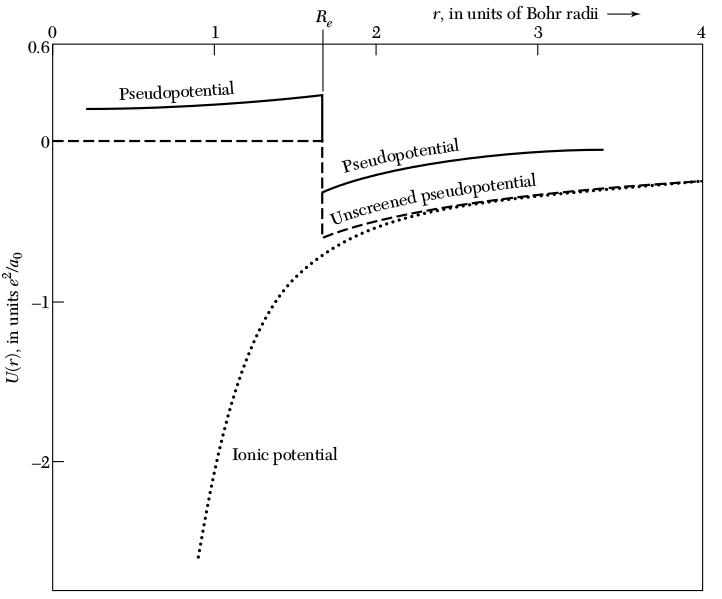
\includegraphics[height=1.60in,width=2.57in,viewport=0 0 980 600,clip]{Pseudo-model-empty_core.png}
\caption{\small \textrm{Pseudopotential for metallic sodium, based on the empty core model and screened by the Thomas-Fermi dielectric function.}}%(与文献\cite{EPJB33-47_2003}图1对比)
\label{Pseudo_model-empty_core}
\end{figure}
加入$\exp(a_4q^4)$因子使得可以适当选择$(a_4<0)$以保证这样赝势的Fourier展开很快收敛。常用半导体材料的赝势参数$a_i$可以从文献\cite{PRB15-2154_1977}得到。这种形式的赝势通常称为软芯(softcore)势。一般说,推导模型赝势要遵从如下三个原则:
\begin{enumerate}
  \item 
要避免引入有大的散射动量$q(q\gg 2k_F)$的平面波作基函数(会引起收敛困难);%与离子赝势在正空间不连续有关。
  \item 
要考虑到赝势的非局域效应;
  \item 
为确定势能参数,尽量使用与金属性质没有直接关联的实验数据。
\end{enumerate}
\begin{figure}[h!]
\centering
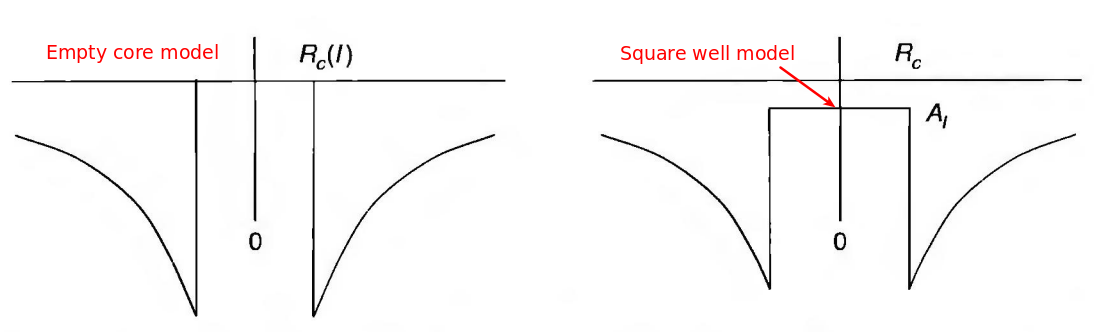
\includegraphics[height=1.30in,width=4.17in,viewport=0 0 1150 350,clip]{Pseudo-model.png}
\caption{\small \textrm{Left:``Empty core'' model potential of Ashcroft in which the potential is zero inside radius $R_c(l)$ which is different for each $l$. Right: Square well model potential with value $A_l$ inside a cut-off radius $R_c$, proposed by Abarenkov and Heine and fit to atomic data by Animalu and Heine..}}% The fact that the potential are weak, zero, or even positive inside cut-off radius $R_c$ is an illustration of the ``cancellation theorem''(与文献\cite{EPJB33-47_2003}图1对比)
\label{Pseudo-model}
\end{figure}

\subsection{模守恒赝势\textrm(Norm-Conserving Pseudo-Poential, NCPP)}
直接构造模型赝势是非常困难的,根据密度泛函理论,自洽的球形屏蔽势和与径向波函数构成Kohn-Sham方程的解,因此可以通过构造合理的赝波函数得到赝势:
\begin{equation}
  \left[-\frac12\frac{d^2}{dr^2}+\frac{l(l+1)}{2r^2}+V(\rho,r)\right]P_{nl}(r)=\varepsilon_{nl}P_{nl}
  \label{eq:solid-103}
\end{equation}
这里$V(\rho,r)$是自洽单电子势$$V(\rho,r)=-Z/r+V_H(\rho,r)+V_{xc}^{LDA}(\rho(r))$$
$V_H(\rho,r)$是Hartree势,$V_{xc}^{LDA}(\rho(r))$是LDA的交换-相关势。

这样得到的赝势称为第一原理赝势,赝势构造的重点由构造赝势本身转移到构造合适的赝波函数。目前使用的电子结构计算的主要赝势方法都是求解全电子波函数,构造相适应的赝函数,再通过径向方程\eqref{eq:solid-103}确定赝势。

绝大部分构造的第一原理赝势满足四个条件\cite{PRB12-4200_1975,PRB18-5449_1978,PRB19-568_1979,PRB20-4082_1979,PRB26-4199_1982,PRL43-1494_1979,JPC13-L189_1980,PRB32-8412_1985,PRB43-1993_1991}:
\begin{itemize}
	\item 首先,由赝势生成的价电子赝波函数不含节点;
	\item 其次,在截断半径$r_{cl}$之外\cite{JPC13-L189_1980,PRB43-1993_1991},具有相同角动量$l$的原子径向赝波函数(pseudo-potential, PP)与全电子波函数(all-electron, AE)相等,%即
\begin{equation}
  P_l^{PP}(r)=P_l^{AE}(r)\quad \mbox{满足}r>r_{cl}
  \label{eq:solid-104}
\end{equation}
或者快速收敛到该值\cite{PRB18-5449_1978,PRL43-1494_1979,PRB32-8412_1985};
	\item 第三,两种波函数在截断半径$r_{cl}$内包含的电荷密度相等\cite{PRL43-1494_1979,PRB43-1993_1991},
\begin{equation}
  \int_0^{r_{cl}}|P_l^{PP}(r)|^2dr=\int_0^{r_{cl}}|P_l^{AE}(r)|^2dr
  \label{eq:solid-105}
\end{equation}
	\item 最后,价态的全电子和赝势的本征值必须相等,$e_l^{PP}=e_l^{AE}$。满足上述全部条件的赝势一般称为模守恒赝势(norm-conserving pseudopotential, NCPP)\cite{PRL43-1494_1979}。有很多方法可以构造出满足上述条件的赝波函数\cite{PRB18-5449_1978,PRB26-4199_1982,PRL43-1494_1979,JPC13-L189_1980,PRB32-8412_1985,PRB43-1993_1991}。得到赝波函数后,逆向求解径向Schr\"odinger方程,可以得到屏蔽(src)赝势:
\begin{equation}
  V_{src,l}^{PP}=\varepsilon_l-\frac{l(l+1)}{2r^2}+\frac1{2P_l^{PP}(r)}\frac{d^2}{dr^2}P_l^{PP}(r)
  \label{eq:solid-106}
\end{equation}
从式\eqref{eq:solid-106}可见,因为赝波函数没有节点,赝势是平缓的,除了原子球心位置不再有其他奇点。
\end{itemize}
\begin{figure}[h!]
\centering
\vspace*{-0.10in}
\includegraphics[height=1.30in,width=4.17in,viewport=0 0 1150 350,clip]{Pseudo-OPW_NCPP.png}
\caption{\small \textrm{Schematic example of a valence function that has the character of a $3s$ orbital near the nucleus and two examples of smooth functions (dashed lines) that equal the full wave-function outside the core region.}}% Left: the smooth part of the valence function defined by OPW-like equation; Right: a smooth pseudo-function that satisfies the norm-conservation condition.(与文献\cite{EPJB33-47_2003}图1对比)
\label{Pseudo-OPW_NCPP}
\end{figure}
由价电子产生的屏蔽与其所处的环境有关,如果扣除价电子屏蔽效应可以得到离子赝势。在自洽迭代过程中利用离子赝势得到特定环境的电子屏蔽。从屏蔽赝势中减去根据赝波函数计算得到的Hartree赝势$V_H^{PP}(r)$和交换-相关赝势$V_{xc}^{PP}(r)$,即离子赝势\cite{PRB43-1993_1991}:
$$V_{ion,H}^{PP}(r)=V_{src,H}^{PP}(r)-V_H^{PP}(r)-V_{xc}^{PP}(r)$$
赝波函数的每个角动量分量有不同的势能,离子赝势算符可以写成:
\begin{equation}
  \hat V_{ion}^{PP}(r)=V_{ion,local}^{PP}+\sum_lV_{nonlocal,l}(r)\hat P_l
  \label{eq:solid-107}
\end{equation}
这里$V_{ion,local}^{PP}(r)$是局域势,$V_{nonlocal,l}(r)=V_{ion,l}^{PP}(r)-V_{ion,local}^{PP}(r)$是角动量$l$的非局域(或半局域)势。$\hat P_l$是投影算符,从波函数中投影出角动量的$l$分量。

Kleinman和Bylander(KB)\cite{PRL48-1425_1982}提出将半局域势\eqref{eq:solid-107}变换为非局域形式的过程:
$$V_{nonlocal,l}^{KB}=\dfrac{|V_{nonlocal,l}(r)\Phi_l^{PP,0}(r)\rangle\langle\Phi_l^{PP,0}(r)V_{nonlocal,l}(r)|}{\langle\Phi_l^{PP,0}(r)|V_{nonlocal,l}(r)|\Phi_l^{PP,0}(r)\rangle}$$
这里$V_{nonlocal,l}(r)$是半局域势[式\eqref{eq:solid-107}],$\Phi_l^{PP,0}(r)$是用以计算赝势的原子角动量$l$的参考赝波函数。选择特定的非局域表象,可以很大程度上节省计算时间。

\subsection{超软赝势\textrm{(Ultra-Soft Pseudo-Potential, USPP)}}
赝势构造的模守恒条件很好地解决了赝势可移植性问题,但对$1s$、$2p$、$3d$等轨道,因为径向波函数本身没有节点,用模守恒方案获得的赝势过于“硬”,所需平面波基组依然非常大。\textrm{Vanderbilt}提出的超软\textrm{(Ultra-soft)}赝势\cite{PRB41-7892_1990},解除了模守恒约束,实现对$1s$、$2p$、$3d$为价电子元素的高效计算。
\begin{figure}[h!]
\centering
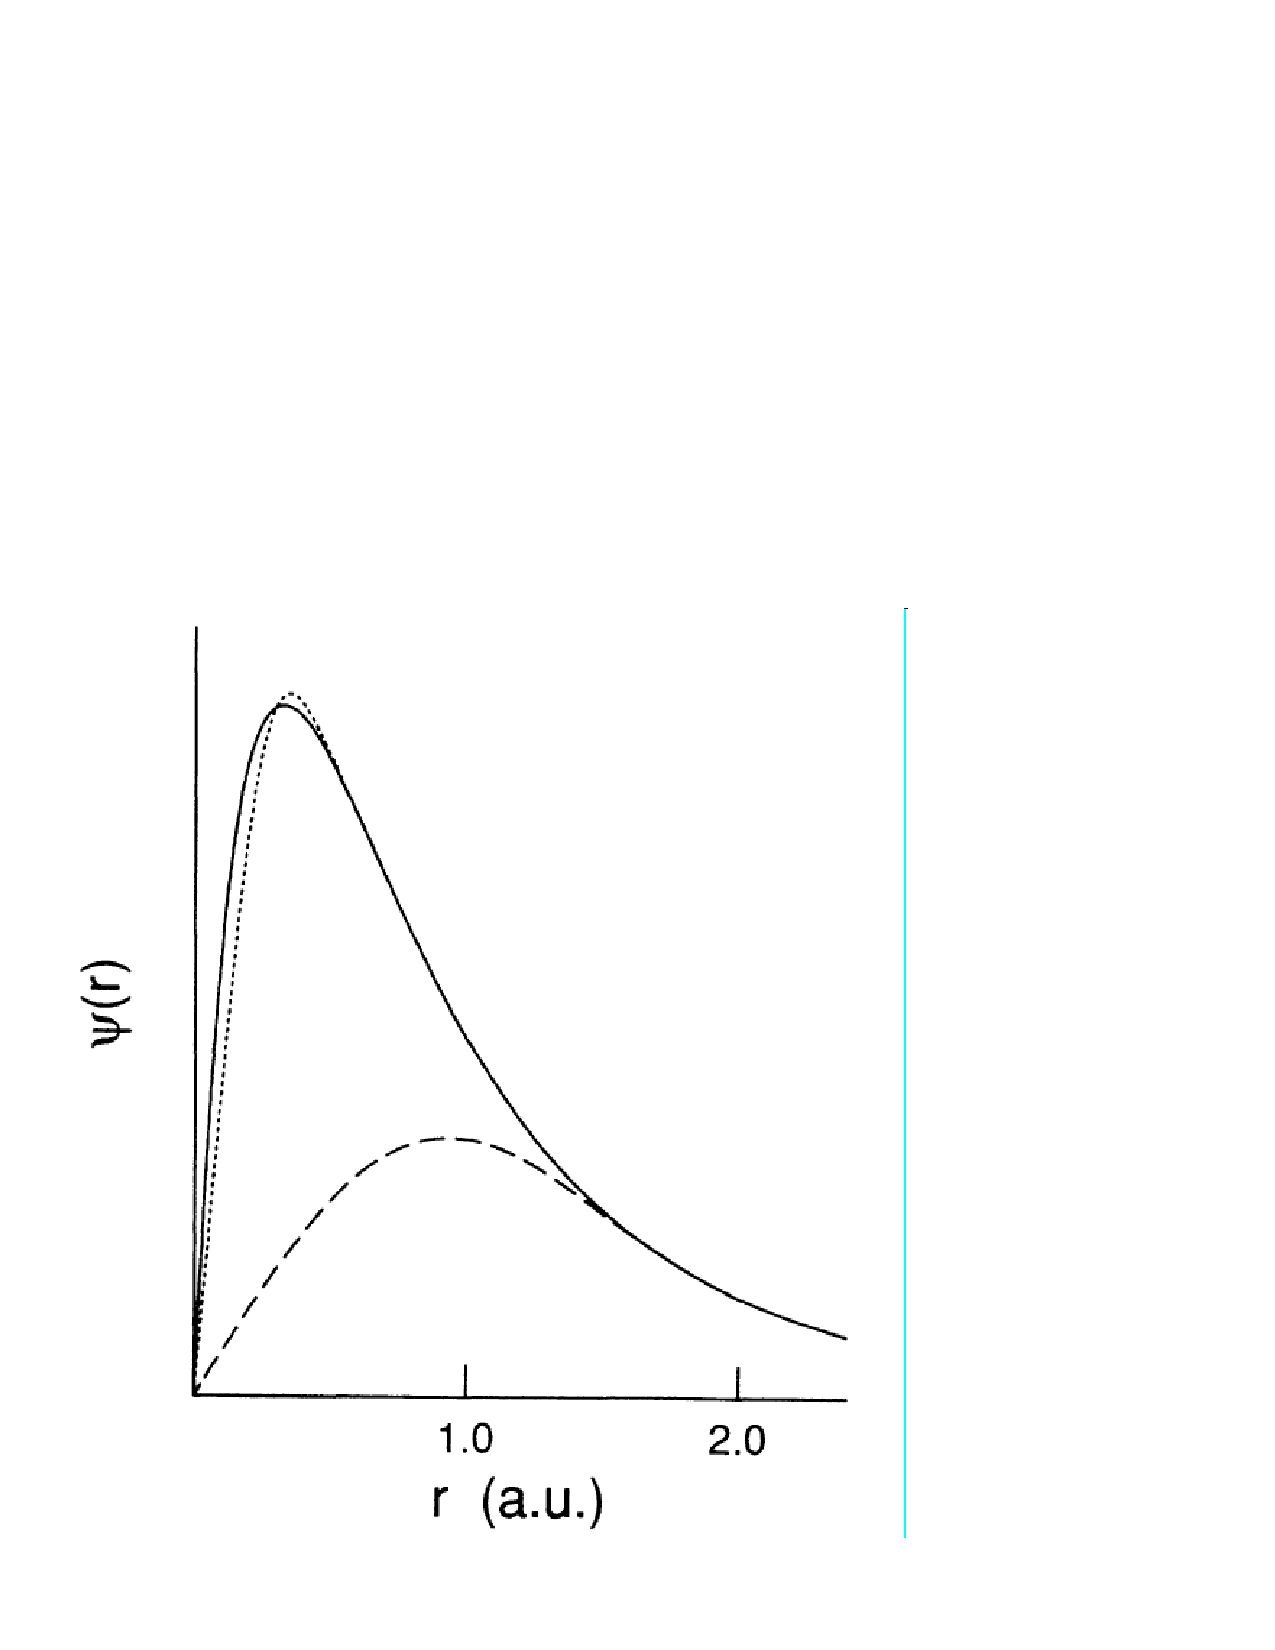
\includegraphics[height=1.35in,width=1.40in,viewport=30 55 415 500,clip]{Norm-US-wave.pdf}
\caption{\small \textrm{Oxygen 2} \textit{p} \textrm{radical wave function (solid), NC-pseudo-wave (dottde) and US-pseudo-wave (dashed).}}%(与文献\cite{EPJB33-47_2003}图1对比)
\label{Norm-US-wave}
\end{figure}

根据Vanderbilt的建议,对$1s$、$2p$、$3d$这种径向不包含节点的价电子波函数,构造赝波函数时放弃模守恒条件,只使用少量平面波基组,但是记录赝波函数与真实波函数的电荷密度差。\footnote{模守恒约束下,赝势\textrm{Schr\"odinger~}方程是标准本征值问题;放弃模守恒条件,引入电荷密度差,可将\textrm{Schr\"odinger}方程表示为广义本征值问题。}策略上,这是通过少量增加的电荷密度差计算为代价(以保持赝势的可移植性),换取基函数规模的大大减少。
\begin{equation}
	Q_{nm}(\vec r)=\varphi_n^{\ast}(\vec r)\varphi_m(\vec r)-\tilde\varphi_n^{\ast}(\vec r)\tilde\varphi_m(\vec r)
  \label{eq:uspp_4}
\end{equation}
超软赝势方法的实现:
\begin{enumerate}
	\item 在平缓的局域势函数$V^L(\vec r)$和赝波函数$|\phi_{lmj}(\vec r)\rangle$的基础上,构造辅助函数
\begin{equation}
	|\chi_{lmj}(\vec r)\rangle=\bigg[\varepsilon_{lj}-\dfrac12\nabla^2-V^L(\vec r)\bigg]|\phi_{lmj}(\vec r)\rangle
  \label{eq:uspp_1}
\end{equation}
	\item 引入矩阵$\mathbf{D}_{ij}=\langle\phi_i|\chi_j\rangle$和局域函数
\begin{equation}
	|\beta_i\rangle=\sum_j(\mathbf{D}^{-1})_{ji}|\chi_{j}\rangle
  \label{eq:uspp_2}
\end{equation}
	\item 与模守恒赝势类似,非局域赝势部分可由$\mathbf{D}$和$\beta_i$表示
\begin{equation}
	V_{NL}=\dfrac{|\chi_i\rangle\langle\chi_i|}{\langle\chi_i|\phi_i\rangle}=\sum_{i,j}\mathbf{D}_{ij}|\beta_i\rangle\langle\beta_j|
  \label{eq:uspp_3}
\end{equation}
\end{enumerate}
根据DFT的总能计算表达式
	\begin{equation}
		\begin{aligned}
			E_{\mathrm{total}}=&\sum_j^{\mathrm{occ}}\langle\phi_{lmj}|\bigg[-\dfrac12\nabla^2+V_{\mathrm{local}}^{\mathrm{ion}}+\sum_{s,s^{\prime}}\mathbf{D}_{s,s^{\prime}}^{\mathrm{ion}}|\beta_s\rangle\langle\beta_{s^{\prime}}|\bigg]|\phi_{lmj}\rangle\\
			&+E_{H}[n_v]+E_{N-N}+E_{XC}[n_v]
		\end{aligned}
  \label{eq:uspp_5}
	\end{equation}
其中$n_v(\vec r)=\sum\limits_j^{\mathrm{occ}}\phi_{lmj}^{\ast}(\vec r)\phi_{lmj}(\vec r)+\sum\limits_{s,s^{\prime}}\sum\limits_j^{\mathrm{occ}}\langle\phi_{lmj}|\beta_{s^{\prime}}\rangle\langle\beta_s|\phi_{lmj}\rangle Q_{s,s^{\prime}}(\vec r)$
	$$V_{\mathrm{local}}^{\mathrm{ion}}=V_{local}-V_{\mathrm H}-V_{XC}$$
	$$\mathbf{D}_{s,s^{\prime}}^{\mathrm{ion}}=\mathbf{D}_{s,s^{\prime}}-\int\mathrm{d}\vec r\big[V_{\mathrm{H}}(\vec r)+V_{XC}(\vec r)\big]Q_{s,s^{\prime}}(r)$$
可以得到广义本征值方程
	$$\bigg[-\dfrac12\nabla^2+V_{\mathrm{local}}+V_{NL}^{\mathrm{US}}-\varepsilon_i\bigg(\mathbf{1}+\sum_{s,s^{\prime}}Q_{s,s^{\prime}}|\beta_s\rangle\langle\beta_{s^{\prime}}|\bigg)\bigg]|\phi_{lmi}\rangle=0$$
